%% Преамбула TeX-файла

% 1. Стиль и язык
\documentclass[utf8x]{G7-32} % Стиль (по умолчанию будет 14pt)
\usepackage[T2A]{fontenc}
\usepackage[russian]{babel}
\usepackage{rotating}
% Остальные стандартные настройки убраны в preamble.inc.tex.
\sloppy

% Настройки стиля ГОСТ 7-32
% Для начала определяем, хотим мы или нет, чтобы рисунки и таблицы нумеровались в пределах раздела, или нам нужна сквозная нумерация.
\EqInChapter % формулы будут нумероваться в пределах раздела
\TableInChapter % таблицы будут нумероваться в пределах раздела
\PicInChapter % рисунки будут нумероваться в пределах раздела

% Добавляем гипертекстовое оглавление в PDF
\usepackage[
bookmarks=true, colorlinks=true, unicode=true,
urlcolor=black,linkcolor=black, anchorcolor=black,
citecolor=black, menucolor=black, filecolor=black,
]{hyperref}

% Изменение начертания шрифта --- после чего выглядит таймсоподобно.
% apt-get install scalable-cyrfonts-tex

\IfFileExists{cyrtimes.sty}
    {
        \usepackage{cyrtimespatched}
    }
    {
        % А если Times нету, то будет CM...
    }

\usepackage{graphicx}   % Пакет для включения рисунков

% С такими оно полями оно работает по-умолчанию:
% \RequirePackage[left=20mm,right=10mm,top=20mm,bottom=20mm,headsep=0pt]{geometry}
% Если вас тошнит от поля в 10мм --- увеличивайте до 20-ти, ну и про переплёт не забывайте:
\geometry{right=20mm}
\geometry{left=30mm}


% Пакет Tikz
\usepackage{tikz}
\usetikzlibrary{arrows,positioning,shadows}

% Произвольная нумерация списков.
\usepackage{enumerate}

% ячейки в несколько строчек
\usepackage{multirow}

% itemize внутри tabular
\usepackage{paralist,array}


% Настройки листингов.
% 8 Листинги

\usepackage{listings}

% Значения по умолчанию
\lstset{
  basicstyle= \footnotesize,
  breakatwhitespace=true,% разрыв строк только на whitespacce
  breaklines=true,       % переносить длинные строки
%   captionpos=b,          % подписи снизу -- вроде не надо
  inputencoding=koi8-r,
  numbers=left,          % нумерация слева
  numberstyle=\footnotesize,
  showspaces=false,      % показывать пробелы подчеркиваниями -- идиотизм 70-х годов
  showstringspaces=false,
  showtabs=false,        % и табы тоже
  stepnumber=1,
  tabsize=4,              % кому нужны табы по 8 символов?
  frame=single
}

% Стиль для псевдокода: строчки обычно короткие, поэтому размер шрифта побольше
\lstdefinestyle{pseudocode}{
  basicstyle=\small,
  keywordstyle=\color{black}\bfseries\underbar,
  language=Pseudocode,
  numberstyle=\footnotesize,
  commentstyle=\footnotesize\it
}

% Стиль для обычного кода: маленький шрифт
\lstdefinestyle{realcode}{
  basicstyle=\scriptsize,
  numberstyle=\footnotesize
}

% Стиль для коротких кусков обычного кода: средний шрифт
\lstdefinestyle{simplecode}{
  basicstyle=\footnotesize,
  numberstyle=\footnotesize
}

% Стиль для BNF
\lstdefinestyle{grammar}{
  basicstyle=\footnotesize,
  numberstyle=\footnotesize,
  stringstyle=\bfseries\ttfamily,
  language=BNF
}

% Определим свой язык для написания псевдокодов на основе Python
\lstdefinelanguage[]{Pseudocode}[]{Python}{
  morekeywords={each,empty,wait,do},% ключевые слова добавлять сюда
  morecomment=[s]{\{}{\}},% комменты {а-ля Pascal} смотрятся нагляднее
  literate=% а сюда добавлять операторы, которые хотите отображать как мат. символы
    {->}{\ensuremath{$\rightarrow$}~}2%
    {<-}{\ensuremath{$\leftarrow$}~}2%
    {:=}{\ensuremath{$\leftarrow$}~}2%
    {<--}{\ensuremath{$\Longleftarrow$}~}2%
}[keywords,comments]

% Свой язык для задания грамматик в BNF
\lstdefinelanguage[]{BNF}[]{}{
  morekeywords={},
  morecomment=[s]{@}{@},
  morestring=[b]",%
  literate=%
    {->}{\ensuremath{$\rightarrow$}~}2%
    {*}{\ensuremath{$^*$}~}2%
    {+}{\ensuremath{$^+$}~}2%
    {|}{\ensuremath{$|$}~}2%
}[keywords,comments,strings]

% Подписи к листингам на русском языке.
\renewcommand\lstlistingname{\cyr\CYRL\cyri\cyrs\cyrt\cyri\cyrn\cyrg}
\renewcommand\lstlistlistingname{\cyr\CYRL\cyri\cyrs\cyrt\cyri\cyrn\cyrg\cyri}


% Полезные макросы листингов.
% Любимые команды
\newcommand{\Code}[1]{\textbf{#1}}


\begin{document}
	
	\frontmatter % выключает нумерацию ВСЕГО; здесь начинаются ненумерованные главы: реферат, введение, глоссарий, сокращения и прочее.
	
	% Команды \breakingbeforechapters и \nonbreakingbeforechapters
	% управляют разрывом страницы перед главами.
	% По-умолчанию страница разрывается.
	
	% \nobreakingbeforechapters
	% \breakingbeforechapters
	
	
	\tableofcontents
	
	\section{Актуальность}
Жизнь человека напрямую зависит от факторов окружающей среды: рельефа, температуры, влажности воздуха, наличия водоёмов, уровня загрязнения и других природных и антропогенных характеристик. 
Изучение и учёт этих факторов играют критическую роль при выборе места жительства, ведения хозяйства и планирования экономической деятельности.

С древнейших времён человечество стремилось обосноваться в наиболее благоприятных регионах.
Однако в силу большого разнообразия климатических зон, географических условий и изменчивости экологических показателей, задача выбора оптимального места остаётся сложной и многомерной. 
В современном мире этот выбор осложняется глобальными изменениями климата, урбанизацией, ростом загрязнения окружающей среды и увеличением мобильности населения, включая рост числа цифровых кочевников — удалённых работников, не привязанных к конкретной географической локации.

Современные реалии требуют наличия цифровых инструментов, которые позволили бы агрегировать, визуализировать и анализировать разнородные геоданные для поддержки принятия решений. 
Создание сервиса, наглядно отображающего ключевые характеристики выбранного региона, отвечает вызовам времени и может использоваться в широком спектре задач:
\begin{itemize}
	\item Обычными пользователями — для подбора комфортных для жизни регионов с учётом климата, экологии и инфраструктуры;
	\item Цифровыми кочевниками — для сравнения условий в разных регионах мира по заданным критериям;
	\item Научными организациями — для изучения изменений климата;
	\item Экологическими фондами — для мониторинга загрязнений и охраны окружающей среды;
	\item Недропользователями и геологоразведочными компаниями — для оценки перспективности территорий с точки зрения наличия полезных ископаемых.
\end{itemize}

Таким образом, разработка такого сервиса является актуальной и востребованной задачей, лежащей на пересечении информационных технологий, географии, экологии.
	
	\mainmatter % это включает нумерацию глав и секций в документе ниже
	
	\chapter{Анализ математической модели}
\section{Аналитическое решение}
Очевидным точным решением является смещенный профиль волны.
\[
	u(x,t) = \phi(x_{0} - vt)
\]

\section{Численное решение}
Система (\ref{eq:sys}) является системой обыкновенного дифференциального уравнения в частных производных.
Для численного решения применяется методы конечных разностей\cite{Turchak2003}. Введём равномерную сетку:
\[
x_i = i \Delta x, \quad t^j = j \Delta t, \quad i = 0, \dots, N_x, \quad j = 0, \dots, N_t,
\]
где $\Delta x = \frac{L}{N_x}$, $\Delta t = \frac{T}{N_t}$. Обозначим $u_i^j = u(x_i, t^j)$.

Будем рассматривать три схемы решения: явную\cite{Turchak2003}, неявную\cite{Turchak2003} и "вверх по потоку" \cite{Patankar1984}.
В качетве профилья волны выберем следующую функцию:
\[
	\phi(x) = 4\exp(-100 x^4).
\]
Для простоты используем нулевые граничные условия. 
Скорость $c$ примем 1. Расстояние $L$ равняется 5. Соответственно, максимальное значение времи тоже равно 5.
Шаг по пространству возьмём 0.05, а по времени - 0.001. Такой выбор удовлетворяет условиям устойчивости всех трёх методов (\ref{eq:ust1} - \ref{eq:ust2}) и не требует больших вычислительных ресурсов.






	\chapter{Конструкторский раздел}
\label{cha:design}

В данном разделе проектируется новая всячина.

\section{Архитектура всячины}

\paragraph{Проверка} параграфа. Вроде работает.
\paragraph{Вторая проверка} параграфа. Опять работает.

Вот.

\begin{itemize}
\item Это список с <<палочками>>.
\item Хотя он и не по ГОСТ, кажется.
\end{itemize}

\begin{enumerate}
\item Поэтому для списка, начинающегося с заглавной буквы, лучше список с цифрами.
\end{enumerate}

Формула \ref{F:F1} совершено бессмысленна.

%Кстати, при каких-то условиях <<удавалось>> получить двойный скобки вокруг номеров формул. Вопрос исследуется.

\begin{equation}
a= cb
\label{F:F1}
\end{equation}


Окружение \texttt{cases} опять работает (см. \ref{F:F2}), спасибо И. Короткову за исправления..


\begin{equation}
a= \begin{cases}
 3x + 5y + z, \mbox{если хорошо} \\
 7x - 2y + 4z, \mbox{если плохо}\\
 -6x + 3y + 2z, \mbox{если совсем плохо}
\end{cases}
\label{F:F2}
\end{equation}

\section{Подсистема всякой ерунды}

Культурная вставка dot-файлов через утилиту dot2tex (рис.~\ref{fig:fig02}).

\begin{figure}
  \centering
% [width=0.5\textwidth] --- регулировка ширины картинки
  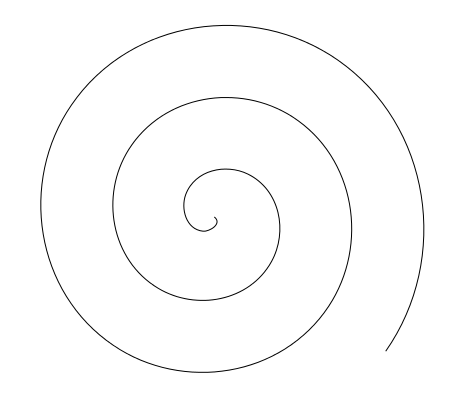
\includegraphics{figures/pic01}
  \caption{Рисунок}
  \label{fig:fig02}
\end{figure}


\subsection{Блок-схема всякой ерунды}

\subsubsection*{Кстати о заголовках}

У нас есть и \Code{subsubsection}. Только лучше её не нумеровать.

%%% Local Variables:
%%% mode: latex
%%% TeX-master: "rpz"
%%% End:

	\chapter{Технологический раздел}
\label{cha:impl}

В данном разделе описано изготовление и требование всячины. Кстати,
в Latex нужно эскейпить подчёркивание (писать <<\verb|some\_function|>> для \Code{some\_function}).

\ifPDFTeX
Для вставки кода есть пакет \Code{listings}. К сожалению, пакет \Code{listings} всё ещё
работает криво при появлении в листинге русских букв и кодировке исходников utf-8.
В данном примере он (увы) на лету конвертируется в koi-8 в ходе сборки pdf.

Есть альтернатива \Code{listingsutf8}, однако она работает лишь с
\Code{\textbackslash{}lstinputlisting}, но не с окружением \Code{\textbackslash{}lstlisting}

Вот так можно вставлять псевдокод (питоноподобный язык определен в \Code{listings.inc.tex}):

\begin{lstlisting}[style=pseudocode,caption={Алгоритм оценки дипломных работ}]
def EvaluateDiplomas():
    for each student in Masters:
        student.Mark := 5
    for each student in Engineers:
        if Good(student):
            student.Mark := 5
        else:
            student.Mark := 4
\end{lstlisting}

Еще в шаблоне определен псевдоязык для BNF:

\begin{lstlisting}[style=grammar,basicstyle=\small,caption={Грамматика}]
  ifstmt -> "if" "(" expression ")" stmt |
            "if" "(" expression ")" stmt1 "else" stmt2
  number -> digit digit*
\end{lstlisting}

В листинге~\ref{lst:sample01} работают русские буквы. Сильная магия. Однако, работает
только во включаемых файлах, прямо в \TeX{} нельзя.

% Обратите внимание, что включается не ../src/..., а inc/src/...
% В Makefile есть соответствующее правило для inc/src/*,
% которое копирует исходные файлы из ../src и конвертирует из UTF-8 в KOI8-R.
% Кстати, поэтому использовать можно только русские буквы и ASCII,
% весь остальной UTF-8 вроде CJK и египетских иероглифов -- нельзя.

\lstinputlisting[language=C,caption=Пример (\Code{test.c}),label=lst:sample01]{listings/test.c}

\else

Для вставки кода есть пакет \texttt{minted}. Он хорош всем кроме: необходимости Python (есть во всех нормальных (нет, Windows, я не про тебя) ОС) и Pygments и того, что нормально работает лишь в \XeLaTeX.

Можно пользоваться расширенным BFN:

\begin{listing}[H]
\begin{ebnfcode}
 letter = "A" | "B" | "C" | "D" | "E" | "F" | "G"
       | "H" | "I" | "J" | "K" | "L" | "M" | "N"
       | "O" | "P" | "Q" | "R" | "S" | "T" | "U"
       | "V" | "W" | "X" | "Y" | "Z" ;
digit = "0" | "1" | "2" | "3" | "4" | "5" | "6" | "7" | "8" | "9" ;
symbol = "[" | "]" | "{" | "}" | "(" | ")" | "<" | ">"
       | "'" | '"' | "=" | "|" | "." | "," | ";" ;
character = letter | digit | symbol | "_" ;
 
identifier = letter , { letter | digit | "_" } ;
terminal = "'" , character , { character } , "'" 
         | '"' , character , { character } , '"' ;
 
lhs = identifier ;
rhs = identifier
     | terminal
     | "[" , rhs , "]"
     | "{" , rhs , "}"
     | "(" , rhs , ")"
     | rhs , "|" , rhs
     | rhs , "," , rhs ;
 
rule = lhs , "=" , rhs , ";" ;
grammar = { rule } ;
\end{ebnfcode}
\caption{EBNF определённый через EBNF}
\label{lst:ebnf}
\end{listing}

А вот в листинге \ref{lst:c} на языке C работают русские комменты. Спасибо Pygments и Minted за это.

\begin{listing}[H]
\cfile{inc/src/test.c}
\caption{Пример — test.c} 
\end{listing}
\label{lst:c}

\fi

% Для вставки реального кода лучше использовать \texttt{\textbackslash lstinputlisting} (который понимает
% UTF8) и стили \Code{realcode} либо \Code{simplecode} (в зависимости от размера куска).




Можно также использовать окружение \Code{verbatim}, если \Code{listings} чем-то не
устраивает. Только следует помнить, что табы в нём <<съедаются>>. Существует так же команда \Code{\textbackslash{}verbatiminput} для вставки файла.

\begin{verbatim}
a_b = a + b; // русский комментарий
if (a_b > 0)
    a_b = 0;
\end{verbatim}

%%% Local Variables:
%%% mode: latex
%%% TeX-master: "rpz"
%%% End:

	\chapter{Построение математической модели}
\section{Модель без термо регулятора}
Основной характеристикой нагревательного прибора является температура. При включенном нагревателе она изменяется со временем. Нас интересует зависимость изменения температуры ($[T]$ = K) от веремни ($[t]=c$): $T(t)$.

Предположим, что нагреватель состоит из одного материала, температура окружающей среды постоянная и равна $T_{env}$. Также отметим, что масса окружающей среды намного больше массы нагревательного прибора (паяльника): $m_{env} >> m_H$ .

Процесс нагревания описыватеся изменением количеством внутренней энергии тела ($\Delta Q$, $[Q]=\text{Дж}$)  от изменении температуры ($\Delta T$):
\begin{equation}
	\Delta Q = cm\Delta T,
	\label{eq:heat_energy}
\end{equation}
где $c$ - удельная теплоёмкость тела $\left(\frac{\text{Дж}}{\text{кг}\cdot\text{К}}\right)$, m - масса нагревателя (кг).

Нагревательный прибор использует электрический ток для увеличения внутренней энергии:
\begin{equation}
	\Delta Q_1 = P \Delta t,
	\label{eq:electrical_energy}
\end{equation}
где $P$ - мощность (Вт).

На изменение внутренней энергии также влияют входящие и исходящие тепловые потоки.
На единицу площади за единицу времени исходящий поток будет изменять энергию на величину $-kT$, 
а входящий - на величину $kT_{env}$, где $k$ - коэффициент теплопередачи, характерынй для данной конструкции нагревательного прибора $\left(\frac{\text{Вт}}{\text{м}^2\text{К}}\right)$. С учётом этих явлений, внутренняя энергия будет изменяться на следующую величину:
\begin{equation}
	\Delta Q_2 = -kS(T-T_{env})\Delta t.
	\label{eq:heat_transfer}
\end{equation}

Кроме этих явлений, согласно закону Стефана-Больцмана, любое тело, нагретое выше абсолютного нуля за единицу веремени на единицу площади излучает энергию равную $-\sigma T^4$, где $\sigma \approx 5.68 \cdot 10 ^{-8} \left(\frac{\text{Вт}}{\text{м}^2\cdot\text{К}^2}\right) $ - постоянная Стефана-Больцмана. Аналогично, излучение поступает из кружающей среды, равное $\sigma T^4_{env}$.
Тогда, измненение внутренней энергии, вызванного этим процессом, равно:
\begin{equation}
	\Delta Q_3 = -\sigma S (T^4 - T^4_{env}) \Delta t.
	\label{eq:stefan_boltzmann}
\end{equation}

Суммируя все потоки энергии, получаем уравнение теплового баланса (см. \ref{eq:heat_energy}, \ref{eq:electrical_energy}, \ref{eq:heat_transfer}, \ref{eq:stefan_boltzmann}):
 
 \begin{equation}
 	cm\Delta T = P\Delta t - k S (T-T_{env})\Delta t - \sigma S (T^4 - T^4_{env})\Delta t .
 	\label{eq:temp_balance}
 \end{equation}
 
 Разделим, обе части уравнения (\ref{eq:temp_balance}) на $cm\Delta t$ и совершим предельный переход $\Delta t \rightarrow 0$:
 \begin{equation}
 	\frac{dT}{dt} = \frac{P - kS(T-T_{env}) - \sigma S (T^4 - T^4_{env})}{cm}
 	\label{eq:dif_temp_balance}
 \end{equation}
 
 Таким образом, мы получили дифференциальное уравнение теплового баланса, которое описывает поведение температуры нагрвателя. 
 Для нахождения единственного достаточно ввести начальное условие: $T(0) = T_0$.
 \section{Модель с терморегулятором}
 
 Для предотвращения перегрева нагревателя, целесообразно установить терморегулятор, которые будет выключать нагреватель при достижении максимальной температуры. 
 Для этого достаточно ввести функцию, которая будет отключать нагреватель, когда температура больше максимально установленной ($T_{max}$), и включать, при достижении минимальной установленной температуры($T_{min})$.
 \begin{equation}
 	I(T, T_{min}, T_{max}) = 
 	\begin{cases}
 		1, & T < T_{min} \\
 		0, & T > T_{max}
 	\end{cases}.
 	\label{eq:switcher}
 \end{equation}
 
 Добавляя (\ref{eq:switcher}) в (\ref{eq:dif_temp_balance}) получим:
  \begin{equation}
 	\frac{dT}{dt} = \frac{P\cdot I(T, T_{min}, T_{max}) - kS(T-T_{env}) - \sigma S (T^4 - T^4_{env})}{cm}
 	\label{eq:dif_temp_balance_with_switcher},
 \end{equation}

 
 
 

	
	\backmatter %% Здесь заканчивается нумерованная часть документа и начинаются ссылки и
	%% заключение
	
	\Conclusion % заключение к отчёту

В результате проделанной работы стало ясно, что ничего не ясно...

%%% Local Variables: 
%%% mode: latex
%%% TeX-master: "rpz"
%%% End: 

	
	% % Список литературы при помощи BibTeX
% Юзать так:
%
% pdflatex rpz
% bibtex rpz
% pdflatex rpz

\bibliographystyle{gost780u}
\bibliography{rpz}

%%% Local Variables: 
%%% mode: latex
%%% TeX-master: "rpz"
%%% End: 
	
	\appendix   % Тут идут приложения
	
	\chapter{Картинки}
\label{cha:appendix1}

\begin{figure}
\centering
\caption{Картинка в приложении. Страшная и ужасная.}
\end{figure}

%%% Local Variables: 
%%% mode: latex
%%% TeX-master: "rpz"
%%% End: 

	\chapter{Еще картинки}
\label{cha:appendix2}

\begin{figure}
\centering
\caption{Еще одна картинка, ничем не лучше предыдущей. Но надо же как-то заполнить место.}
\end{figure}

%%% Local Variables: 
%%% mode: latex
%%% TeX-master: "rpz"
%%% End: 

	
\end{document}

%%% Local Variables:
%%% mode: latex
%%% TeX-master: t
%%% End:
